% ICCIT Fig. 1: study pipeline. Drawn at the true text width (516 pt = 18.14 cm), in the
% paper's own Times face, so body text prints at 7 pt and titles at 8 pt.
% Three bands (Input, Model, Evaluation), orthogonal arrows, tinted fills with
% same-hue borders, one hue per pooling head (reused for the line in Fig. 2).
% Every count printed here is stated in the Methods text; re-check there if it changes.
% Build: pdflatex fig_pipeline_cr.tex  (run in this folder), copy the PDF up one level.
\documentclass[border=1pt]{standalone}
\usepackage{times}
\usepackage{amsmath,amssymb}
\usepackage{xcolor}
\usepackage{tikz}
\usetikzlibrary{arrows.meta}

% neutral structure
\definecolor{slate}{HTML}{4B5663}
\definecolor{band}{HTML}{F3F5F8}
\definecolor{bandline}{HTML}{C9D1DB}
\definecolor{boxline}{HTML}{6B7785}
% one hue per head (Paul Tol bright), tint + same-hue border
\definecolor{gap}{HTML}{4477AA}   \definecolor{gapf}{HTML}{DCE6F1}
\definecolor{gmp}{HTML}{CC3344}   \definecolor{gmpf}{HTML}{F8DDE1}
\definecolor{se}{HTML}{AA3377}    \definecolor{sef}{HTML}{EFDAE6}
\definecolor{gcp}{HTML}{228833}   \definecolor{gcpf}{HTML}{DCEEDF}
\definecolor{bb}{HTML}{6B7785}    \definecolor{bbf}{HTML}{E9ECF0}
% single focal accent: the one thing the study varies (stage 3)
\definecolor{focal}{HTML}{B26B00}  \definecolor{focalf}{HTML}{FFF4E0}

\tikzset{
  >={Stealth[length=4pt,width=3.4pt]},
  flow/.style={draw=slate, line width=0.8pt, rounded corners=1.5pt},
  flowmuted/.style={draw=slate!50, line width=0.8pt, rounded corners=1.5pt},
  stagebox/.style={draw=boxline, line width=0.7pt, fill=white, rounded corners=3pt,
                   inner sep=0pt, align=center},
  badge/.style={circle, fill=slate, text=white, font=\fontsize{6.5}{6.5}\selectfont\bfseries,
                inner sep=0pt, minimum size=0.42cm},
  chip/.style={draw, line width=0.6pt, rounded corners=1.2pt, minimum height=0.38cm,
               font=\fontsize{7}{7}\selectfont\bfseries, inner sep=1.5pt},
  bandlabel/.style={font=\fontsize{7}{8}\selectfont\scshape, text=slate, anchor=north west},
  ttl/.style={font=\fontsize{8.2}{9}\selectfont\bfseries, text=black},
  sub/.style={font=\fontsize{7.2}{8.4}\selectfont, text=black!80},
}
\newcommand{\hchip}[4]{% x y name label  (name = gap|gmp|se|gcp)
  \node[chip, draw=#3, fill=#3f, text=#3!80!black, minimum width=1.05cm] at (#1,#2) {#4};}

\begin{document}
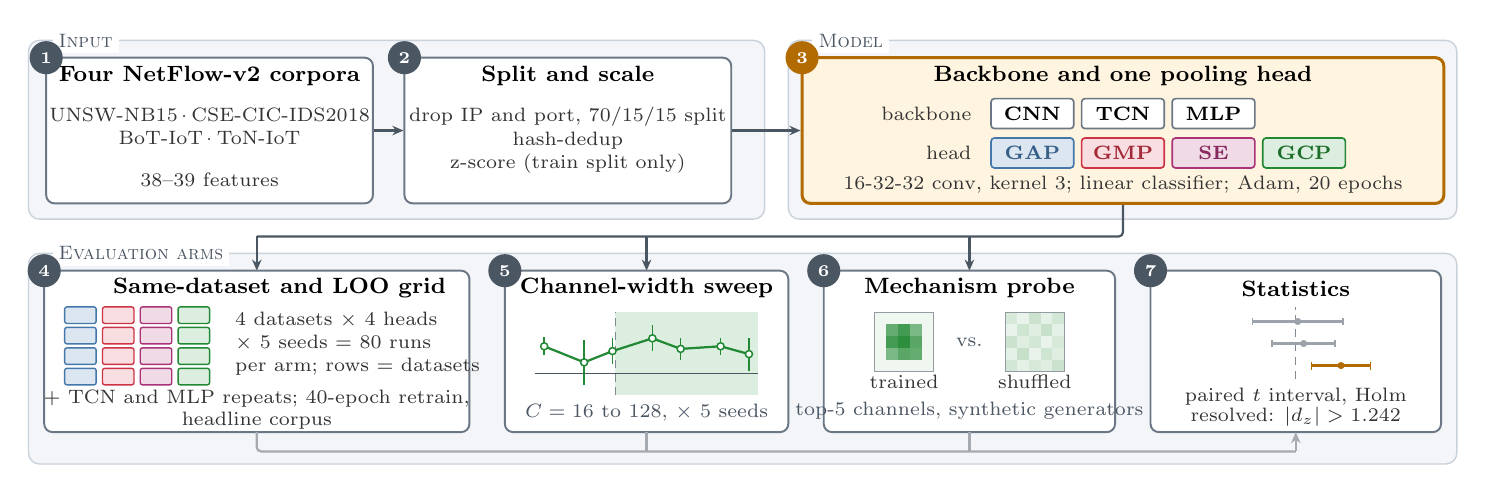
\begin{tikzpicture}[x=1cm,y=1cm]

% ---------------- band panels (legend sits on the top border) ----------------
\fill[band, draw=bandline, line width=0.5pt, rounded corners=4pt] (0,2.98) rectangle (9.35,5.25);
\fill[band, draw=bandline, line width=0.5pt, rounded corners=4pt] (9.65,2.98) rectangle (18.14,5.25);
\fill[band, draw=bandline, line width=0.5pt, rounded corners=4pt] (0,-0.13) rectangle (18.14,2.545);
\node[bandlabel, anchor=west, fill=white, inner sep=2.2pt] at (0.30,5.25) {Input};
\node[bandlabel, anchor=west, fill=white, inner sep=2.2pt] at (9.95,5.25) {Model};
\node[bandlabel, anchor=west, fill=white, inner sep=2.2pt] at (0.30,2.545) {Evaluation arms};

% ---------------- 1 corpora (top row: boxes y 3.60 to 5.45) ----------------
\node[stagebox, minimum width=4.15cm, minimum height=1.85cm] (s1) at (2.30,4.105) {};
\node[ttl] at (2.30,4.800) {Four NetFlow-v2 corpora};
\node[sub, align=center] at (2.30,4.160) {UNSW-NB15\,\textperiodcentered\,CSE-CIC-IDS2018\\BoT-IoT\,\textperiodcentered\,ToN-IoT};
\node[sub] at (2.30,3.480) {38--39 features};
\node[badge] at (0.225,5.030) {1};

% ---------------- 2 split and scale ----------------
\node[stagebox, minimum width=4.15cm, minimum height=1.85cm] (s2) at (6.85,4.105) {};
\node[ttl] at (6.85,4.800) {Split and scale};
\node[sub, align=center] at (6.85,3.980) {drop IP and port, 70/15/15 split\\hash-dedup\\z-score (train split only)};
\node[badge] at (4.775,5.030) {2};
\draw[flow,->] (s1.east) -- (s2.west);

% ---------------- 3 backbone and head ----------------
\node[stagebox, draw=focal, fill=focalf, line width=1.1pt, minimum width=8.15cm, minimum height=1.85cm] (s3) at (13.90,4.105) {};
\node[ttl] at (13.90,4.800) {Backbone and one pooling head};
\node[sub, anchor=east] at (12.10,4.320) {backbone};
\node[chip, draw=bb, fill=white, text=black, minimum width=1.05cm] at (12.75,4.320) {CNN};
\node[chip, draw=bb, fill=white, text=black, minimum width=1.05cm] at (13.90,4.320) {TCN};
\node[chip, draw=bb, fill=white, text=black, minimum width=1.05cm] at (15.05,4.320) {MLP};
\node[sub, anchor=east] at (12.10,3.820) {head};
\hchip{12.75}{3.820}{gap}{GAP}
\hchip{13.90}{3.820}{gmp}{GMP}
\hchip{15.05}{3.820}{se}{SE}
\hchip{16.20}{3.820}{gcp}{GCP}
\node[sub] at (13.90,3.420) {16-32-32 conv, kernel 3; linear classifier; Adam, 20 epochs};
\node[badge, fill=focal] at (9.825,5.030) {3};
\draw[flow,->] (s2.east) -- (s3.west);

% ---------------- fan-out from stage 3 to the arms ----------------
\draw[flow] (s3.south) -- (13.90,2.76) -- (2.90,2.76);
\draw[flow,->] (2.90,2.76) -- (2.90,2.325);
\draw[flow,->] (7.85,2.76) -- (7.85,2.325);
\draw[flow,->] (11.95,2.76) -- (11.95,2.325);

% ---------------- 4 same-dataset x LOO grid (eval boxes y 0.275 to 2.325) ----------------
\node[stagebox, minimum width=5.40cm, minimum height=2.05cm] (s4) at (2.90,1.30) {};
\node[ttl, anchor=west] at (0.95,2.10) {Same-dataset and LOO grid};
% 4x4 chip grid, rows = datasets, columns = heads
\foreach \r in {0,1,2,3}{
  \foreach \c/\h in {0/gap,1/gmp,2/se,3/gcp}{
    \node[draw=\h, fill=\h f, line width=0.5pt, rounded corners=0.8pt, minimum width=0.40cm,
          minimum height=0.21cm, inner sep=0pt] at (0.66+\c*0.48, 1.76-\r*0.26) {};
  }
}
\node[sub, align=left, anchor=west] at (2.50,1.40) {4 datasets $\times$ 4 heads\\$\times$ 5 seeds $=$ 80 runs\\per arm; rows = datasets};
\node[sub, align=center, font=\fontsize{6.8}{7.6}\selectfont] at (2.90,0.56) {+ TCN and MLP repeats; 40-epoch retrain,\\headline corpus};
\node[badge] at (0.20,2.325) {4};

% ---------------- 5 channel-width sweep (mini plot from the real sweep data) ----------------
\node[stagebox, minimum width=3.60cm, minimum height=2.05cm] (s5) at (7.85,1.30) {};
\node[ttl] at (7.85,2.10) {Channel-width sweep};
\fill[gcpf] (7.455,0.74) rectangle (9.270,1.80);
\draw[slate!70, densely dashed, line width=0.5pt] (7.455,0.74) -- (7.455,1.80);
\draw[slate, line width=0.5pt] (6.430,1.020) -- (9.270,1.020);
\draw[gcp, line width=0.8pt] (6.550,1.365) -- (7.057,1.161) -- (7.417,1.304) -- (7.924,1.466) -- (8.283,1.332) -- (8.790,1.365) -- (9.150,1.266);
\draw[gcp, line width=0.55pt] (6.550,1.253) -- (6.550,1.477);
\fill[white, draw=gcp, line width=0.55pt] (6.550,1.365) circle (0.045);
\draw[gcp, line width=0.55pt] (7.057,0.879) -- (7.057,1.443);
\fill[white, draw=gcp, line width=0.55pt] (7.057,1.161) circle (0.045);
\draw[gcp, line width=0.55pt] (7.417,1.144) -- (7.417,1.464);
\fill[white, draw=gcp, line width=0.55pt] (7.417,1.304) circle (0.045);
\draw[gcp, line width=0.55pt] (7.924,1.301) -- (7.924,1.631);
\fill[white, draw=gcp, line width=0.55pt] (7.924,1.466) circle (0.045);
\draw[gcp, line width=0.55pt] (8.283,1.196) -- (8.283,1.468);
\fill[white, draw=gcp, line width=0.55pt] (8.283,1.332) circle (0.045);
\draw[gcp, line width=0.55pt] (8.790,1.260) -- (8.790,1.469);
\fill[white, draw=gcp, line width=0.55pt] (8.790,1.365) circle (0.045);
\draw[gcp, line width=0.55pt] (9.150,1.056) -- (9.150,1.475);
\fill[white, draw=gcp, line width=0.55pt] (9.150,1.266) circle (0.045);
\node[sub, font=\fontsize{6.8}{7.6}\selectfont, text=slate] at (7.85,0.52) {$C=16$ to 128, $\times$ 5 seeds};
\node[badge] at (6.05,2.325) {5};

% ---------------- 6 mechanism probe (schematic icons, no data) ----------------
\node[stagebox, minimum width=3.70cm, minimum height=2.05cm] (s6) at (11.95,1.30) {};
\node[ttl] at (11.95,2.10) {Mechanism probe};
\fill[gcp!7!white] (10.745,1.645) rectangle (10.895,1.795);
\fill[gcp!7!white] (10.895,1.645) rectangle (11.045,1.795);
\fill[gcp!7!white] (11.045,1.645) rectangle (11.195,1.795);
\fill[gcp!7!white] (11.195,1.645) rectangle (11.345,1.795);
\fill[gcp!7!white] (11.345,1.645) rectangle (11.495,1.795);
\fill[gcp!7!white] (10.745,1.495) rectangle (10.895,1.645);
\fill[gcp!70!white] (10.895,1.495) rectangle (11.045,1.645);
\fill[gcp!85!white] (11.045,1.495) rectangle (11.195,1.645);
\fill[gcp!60!white] (11.195,1.495) rectangle (11.345,1.645);
\fill[gcp!7!white] (11.345,1.495) rectangle (11.495,1.645);
\fill[gcp!7!white] (10.745,1.345) rectangle (10.895,1.495);
\fill[gcp!85!white] (10.895,1.345) rectangle (11.045,1.495);
\fill[gcp!95!white] (11.045,1.345) rectangle (11.195,1.495);
\fill[gcp!75!white] (11.195,1.345) rectangle (11.345,1.495);
\fill[gcp!7!white] (11.345,1.345) rectangle (11.495,1.495);
\fill[gcp!7!white] (10.745,1.195) rectangle (10.895,1.345);
\fill[gcp!60!white] (10.895,1.195) rectangle (11.045,1.345);
\fill[gcp!75!white] (11.045,1.195) rectangle (11.195,1.345);
\fill[gcp!70!white] (11.195,1.195) rectangle (11.345,1.345);
\fill[gcp!7!white] (11.345,1.195) rectangle (11.495,1.345);
\fill[gcp!7!white] (10.745,1.045) rectangle (10.895,1.195);
\fill[gcp!7!white] (10.895,1.045) rectangle (11.045,1.195);
\fill[gcp!7!white] (11.045,1.045) rectangle (11.195,1.195);
\fill[gcp!7!white] (11.195,1.045) rectangle (11.345,1.195);
\fill[gcp!7!white] (11.345,1.045) rectangle (11.495,1.195);
\draw[slate!60, line width=0.4pt] (10.745,1.045) rectangle (11.495,1.795);
\fill[gcp!18!white] (12.405,1.645) rectangle (12.555,1.795);
\fill[gcp!10!white] (12.555,1.645) rectangle (12.705,1.795);
\fill[gcp!24!white] (12.705,1.645) rectangle (12.855,1.795);
\fill[gcp!12!white] (12.855,1.645) rectangle (13.005,1.795);
\fill[gcp!20!white] (13.005,1.645) rectangle (13.155,1.795);
\fill[gcp!10!white] (12.405,1.495) rectangle (12.555,1.645);
\fill[gcp!22!white] (12.555,1.495) rectangle (12.705,1.645);
\fill[gcp!14!white] (12.705,1.495) rectangle (12.855,1.645);
\fill[gcp!26!white] (12.855,1.495) rectangle (13.005,1.645);
\fill[gcp!12!white] (13.005,1.495) rectangle (13.155,1.645);
\fill[gcp!24!white] (12.405,1.345) rectangle (12.555,1.495);
\fill[gcp!14!white] (12.555,1.345) rectangle (12.705,1.495);
\fill[gcp!20!white] (12.705,1.345) rectangle (12.855,1.495);
\fill[gcp!10!white] (12.855,1.345) rectangle (13.005,1.495);
\fill[gcp!18!white] (13.005,1.345) rectangle (13.155,1.495);
\fill[gcp!12!white] (12.405,1.195) rectangle (12.555,1.345);
\fill[gcp!26!white] (12.555,1.195) rectangle (12.705,1.345);
\fill[gcp!10!white] (12.705,1.195) rectangle (12.855,1.345);
\fill[gcp!22!white] (12.855,1.195) rectangle (13.005,1.345);
\fill[gcp!14!white] (13.005,1.195) rectangle (13.155,1.345);
\fill[gcp!20!white] (12.405,1.045) rectangle (12.555,1.195);
\fill[gcp!12!white] (12.555,1.045) rectangle (12.705,1.195);
\fill[gcp!18!white] (12.705,1.045) rectangle (12.855,1.195);
\fill[gcp!14!white] (12.855,1.045) rectangle (13.005,1.195);
\fill[gcp!24!white] (13.005,1.045) rectangle (13.155,1.195);
\draw[slate!60, line width=0.4pt] (12.405,1.045) rectangle (13.155,1.795);
\node[sub, font=\fontsize{6.8}{7.6}\selectfont, text=slate] at (11.95,1.42) {vs.};
\node[sub, font=\fontsize{6.8}{7.6}\selectfont] at (11.12,0.92) {trained};
\node[sub, font=\fontsize{6.8}{7.6}\selectfont] at (12.78,0.92) {shuffled};
\node[sub, font=\fontsize{6.8}{7.6}\selectfont, text=slate] at (11.95,0.55) {top-5 channels, synthetic generators};
\node[badge] at (10.10,2.325) {6};

% ---------------- 7 statistics (schematic icon, no data) ----------------
\node[stagebox, minimum width=3.69cm, minimum height=2.05cm] (s7) at (16.095,1.30) {};
\node[ttl] at (16.095,2.10) {Statistics};
\draw[slate!70, densely dashed, line width=0.5pt] (16.095,0.95) -- (16.095,1.86);
\draw[slate!55, line width=0.8pt] (15.545,1.68) -- (16.695,1.68);
\draw[slate!55, line width=0.6pt] (15.545,1.63) -- (15.545,1.73);
\draw[slate!55, line width=0.6pt] (16.695,1.63) -- (16.695,1.73);
\fill[slate!55] (16.120,1.68) circle (0.045);
\draw[slate!55, line width=0.8pt] (15.795,1.4) -- (16.595,1.4);
\draw[slate!55, line width=0.6pt] (15.795,1.3499999999999999) -- (15.795,1.45);
\draw[slate!55, line width=0.6pt] (16.595,1.3499999999999999) -- (16.595,1.45);
\fill[slate!55] (16.195,1.4) circle (0.045);
\draw[focal, line width=0.8pt] (16.295,1.12) -- (17.045,1.12);
\draw[focal, line width=0.6pt] (16.295,1.07) -- (16.295,1.1700000000000002);
\draw[focal, line width=0.6pt] (17.045,1.07) -- (17.045,1.1700000000000002);
\fill[focal] (16.670,1.12) circle (0.045);
\node[sub, font=\fontsize{6.8}{7.6}\selectfont] at (16.095,0.72) {paired $t$ interval, Holm};
\node[sub, font=\fontsize{6.8}{7.6}\selectfont] at (16.095,0.47) {resolved: $|d_z|>1.242$};
\node[badge] at (14.25,2.325) {7};

% arms feed the statistics through a bottom bus
\draw[flowmuted] (2.90,0.275) -- (2.90,0.03) -- (16.095,0.03);
\draw[flowmuted] (7.85,0.275) -- (7.85,0.03);
\draw[flowmuted] (11.95,0.275) -- (11.95,0.03);
\draw[flowmuted,->] (16.095,0.03) -- (16.095,0.275);
\end{tikzpicture}
\end{document}
